\documentclass[a4paper,parskip=half,10pt,bibtotoc,abstracton,oneside,noindent,DIV15]{scrartcl}
\usepackage{url,textcomp}
\usepackage{listings}
\usepackage{pslatex,color,hyperref,graphicx,titlesec}
\usepackage[OT1]{fontenc}

\titlespacing{\section}{0pt}{*2}{*0.5}

\setlength{\parindent}{0pt}

\title{SeqPig Manual}

\definecolor{lightlightgray}{gray}{0.9}
\definecolor{OliveGreen}{cmyk}{0.64,0,0.95,0.40}

%\usepackage{tex4ht}
\newcommand{\Css}[1]{}

\lstset{
language=C,                             % Code langugage
basicstyle=\ttfamily,                   % Code font, Examples: \footnotesize, \ttfamily
keywordstyle=\color{OliveGreen},        % Keywords font ('*' = uppercase)
commentstyle=\color{gray},              % Comments font
%numbers=left,                           % Line nums position
%numberstyle=\tiny,                      % Line-numbers fonts
%stepnumber=1,                           % Step between two line-numbers
%numbersep=5pt,                          % How far are line-numbers from code
backgroundcolor=\color{lightlightgray}, % Choose background color
frame=none,                             % A frame around the code
tabsize=2,                              % Default tab size
captionpos=b,                           % Caption-position = bottom
breaklines=true,                        % Automatic line breaking?
breakatwhitespace=false,                % Automatic breaks only at whitespace?
showspaces=false,                       % Dont make spaces visible
showtabs=false,                         % Dont make tabls visible
columns=flexible,                       % Column format
morekeywords={__global__, __device__},  % CUDA specific keywords
upquote=true,
}

\lstset{breaklines=true}

\Css{div.lstlisting{font-family: monospace;
    white-space: nowrap; margin-top:0.5em;
    margin-bottom:0.5em;
    color: blue;}}

\Css{ol li { padding: 0; margin: 0.5em; }}

\begin{document}

\maketitle

\tableofcontents
\newpage

\section{Introduction}

SeqPig is a library for Apache Pig \url{http://pig.apache.org/} for the
distributed analysis of large sequencing datasets on Hadoop clusters.  With
SeqPig one can easily take advantage of the advanced high-level features of Pig
to manipulate and analyze sequencing data, thus writing simple scripts that
automatically run as scalable distributed programs on potentially very large
Hadoop clusters.

SeqPig provides a number of features and functionalities.  It provides import
and export functions for file formats commonly used in bioinformatics, as well
as a collection of Pig user-defined-functions (UDF's) that add to Pig
functionality specifically designed for processing aligned and unaligned
sequencing data. Currently SeqPig supports BAM, SAM, FastQ and Qseq input and
output, thanks in part to the functionality provided by the Hadoop-BAM library.

This document can also be found under
\url{http://seqpig.sourceforge.net/}.\\ Contact information:
\url{mailto:seqpig-users@lists.sourceforge.net}

Releases of SeqPig come bundled with Picard/Samtools, which is
developed at the Wellcome Trust Sanger Institute, and Seal, which
is developed
at CRS4. See\\
\url{http://samtools.sourceforge.net/} and 
\url{http://biodoop-seal.sourceforge.net/}
for more details.


\section{Installation}

\Css{div.lstlisting{font-family: monospace;
    white-space: nowrap; margin-top:0.5em;
    margin-bottom:0.5em;
    color: blue;}}

\Css{ol li { padding: 0; margin: 0.5em; }}

\subsection{Dependencies}

\begin{itemize}
	\item A Hadoop cluster (we have tested with Hadoop 0.20.2)
	\item Pig (at least version 0.10)
\end{itemize}
%
The following two dependencies are already included in a pre-compiled SeqPig release:
\begin{itemize}
\item Hadoop-BAM (\url{https://sourceforge.net/projects/hadoop-bam/})
\item Seal (\url{http://biodoop-seal.sourceforge.net/})
\end{itemize}

\subsection{Environment variables}
\label{sect:install_env}
\begin{itemize}
\item Set Hadoop-related variables (e.g., {\tt HADOOP\_HOME}) for your
	installation
\item Set {\tt PIG\_HOME} to point to your Pig installation
\end{itemize}

On a Cloudera Hadoop installation with Pig a suitable environment configuration would be:
\begin{lstlisting} 
$ export HADOOP_HOME=/usr/lib/hadoop
$ export PIG_HOME=/usr/lib/pig
\end{lstlisting}

\subsection{Installing a pre-compiled release}

\begin{enumerate}
\item Dowload the latest SeqPig release from \url{https://sourceforge.net/projects/seqpig/}
\item Untar the release into an installation directory of your choice and set the {\tt SEQPIG\_HOME}
  environment variable to point to the installation directory of SeqPig; e.g.,
%
\begin{lstlisting} 
$ tar xvzf seqpig_0.5.tar.gz -C /usr/local/java/
$ export SEQPIG_HOME=/usr/local/java/seqpig 
\end{lstlisting}
%
\item For your convenience, you can add the bin directory to your {\tt PATH}:
%
\begin{lstlisting} 
$ export PATH=${PATH}:${SEQPIG_HOME}/bin
\end{lstlisting}
%
This way, you'll be able to start a SeqPig-enabled Pig shell by running the {\tt
seqpig} command.
\end{enumerate}

\subsection{Instructions for building SeqPig}

\begin{enumerate}
\item Download hadoop-bam from \url{https://sourceforge.net/projects/hadoop-bam/}.
\item Download and build the latest Seal git master version from
 \url{http://biodoop-seal.sourceforge.net/}. Note that this requires setting
 {\tt HADOOP\_BAM} to the installation directory of hadoop-bam.

\item Inside the cloned SeqPig git repository create a
{\tt lib/} subdirectory and copy (or link) the jar files
from hadoop-bam and Seal to this new directory.  The files should be:
\begin{enumerate}
	\item \verb@${HADOOP_BAM}/*.jar@
	\item from the Seal directory, run \verb@ find build/ -name seal.jar@
\end{enumerate}
%
Note: the Picard and Sam jar files are contained in the hadoop-bam release
for convenience.

\item Run {\tt ant} to build {\tt SeqPig.jar}.
\end{enumerate}

Once you've built SeqPig, you can move the directory to a location of your
preference (if on a shared system, perhaps {\tt /usr/local/java/seqpig}, else
even your home directory could be fine).

\subsubsection{Note}
\label{sect:piggybank_note}

Some of the example scripts in this manual (e.g.,
Section~\ref{sect:read_clipping}) require functions from \emph{PiggyBank},
which is a collection of publicly available User-Defined Functions (UDF's)
that are distributed with Pig but may need to be built separately, depending on
your Pig distribution.
For more details see
\url{https://cwiki.apache.org/confluence/display/PIG/PiggyBank}. Verify that
PiggyBank has been compiled by looking for the file {\tt piggybank.jar} under
{\tt \$PIG\_HOME}:
\begin{lstlisting} 
$ find $PIG_HOME -name piggybank.jar
\end{lstlisting}
If PiggyBank hasn't been compiled, go into {\tt
\$PIG\_HOME/contrib/piggybank/java} and run {\tt ant}.

\subsection{Running on Amazon Elastic MapReduce}

Assuming you have started an interactive Pig Job Flow (for example via
the AWS console), you can login into the master node and copy the SeqPig release to the Hadoop
user home directory. Then set both {\tt SEQPIG\_HOME} and {\tt PIG\_HOME}
correctly ({\tt HADOOP\_HOME} should be set by default). Note that the
Pig version installed does not necessarily match the latest Pig release.
The advantage, however, is the ability to use S3 buckets for input and
output.

Consider the following example for starting SeqPig on EMR. In this example we assume that the SeqPig release was installed
into {\tt /home/hadoop/seqpig}.
\begin{lstlisting} 
$ export SEQPIG_HOME=/home/hadoop/seqpig
$ export PIG_HOME=/home/hadoop/.versions/pig-0.9.2
$ /home/hadoop/seqpig/bin/seqpig
\end{lstlisting}

\subsection{Tests}

After building SeqPig it may be a good idea to run tests to verify that
the environment has been set up correctly. When inside the SeqPig directory
execute
\begin{lstlisting} 
$ test/test_all.sh
\end{lstlisting}
By default the tests run Pig in local mode. In order to test Hadoop
mode pass the command line argument {\tt -h}. Note that this test
requires that Hadoop to be set up correctly. It first imports a BAM
file, sorts the reads by coordinate and converts it to SAM for
comparing the results. The test should end with the line
\begin{lstlisting}
TEST: all tests passed
\end{lstlisting}
If you intend to run SeqPig on an Amazon Elastic MapReduce instance, you can
also test input from S3 by providing an S3 path to the file {\tt data/input.bam}:
\begin{lstlisting} 
$ test/test_all.sh -s <s3_path>
\end{lstlisting}
for example:
\begin{lstlisting} 
$ test/test_all.sh -s seqpig/data/input.bam
\end{lstlisting}
where {\tt seqpig} is the name of the S3 bucket.

\subsection{Usage}

\subsubsection{Pig grunt shell for interactive operations}
Assuming that all the environment variables have been set as described in the
previous sections, you can start the SeqPig-enabled ``grunt'' shell by running
%
\begin{lstlisting}
$ seqpig
\end{lstlisting}
%
If you prefer to tun SeqPig in local mode (without Hadoop), which is useful
for debugging scripts, you can start it by running
%
\begin{lstlisting}
$ seqpig -x local
\end{lstlisting}
%
\subsubsection{Starting scripts from the command line for non-interactive use}
Alternatively to using the interactive Pig grunt shell, users can write scripts
that are then submitted to Pig/Hadoop for automated execution. This type of
execution has the advantage of being able to handle parameters; for instance,
one can parametrize input and output files. See the {\tt /scripts} directory
inside the SeqPig distribution and Section \ref{sect:examples} for examples.



\section{Examples}
\label{sect:examples}

This section lists a number of examples of the types of operations
that can be performed with SeqPig. Each example is typically a mix of
standard Pig operations and SeqPig user-defined functions (UDF's).
Note that once the data has been imported to Pig the only difference
between, say, read data originating from BAM and Fastq files, is that
some fields in tuples derived from BAM may not be available in those
from Fastq, e.g., alignment start positions.

\subsection{Operations on BAM files}

To access sequencing data in BAM files, SeqPig uses Hadoop-BAM, which
provides access to all fields and optional attributes in the data
records. All the examples below assume that an input BAM file is
initially imported to HDFS via
\begin{lstlisting} 
$ prepareBamInput.sh input.bam
\end{lstlisting} 
This additional setup step is required to extract the header and store
it inside HDFS to simplify some operations that only operate on a
chunk of the BAM file without having access to the original header.
Similarly, for uncompressed SAM files there is a corresponding {\tt
prepareSamInput.sh}. Once the input file is imported into HDFS it
can be loaded in the grunt shell via
\begin{lstlisting} 
A = load 'input.bam' using BamLoader('yes');
\end{lstlisting} 
The 'yes' parameter to {\tt BamLoader} chooses read attributes to be
loaded; choose 'no' whenever these are not required).

Once some operations have been performed, the resulting (possibly
modified) read data can then be stored into a new BAM file via
\begin{lstlisting}
store A into 'output.bam' using BamStorer('input.bam.asciiheader');
\end{lstlisting}
and can also be exported from HDFS to the local filesystem via
\begin{lstlisting}
prepareBamOutput.sh output.bam
\end{lstlisting}
\begin{description}
	\item[Note] The Pig store operation requires a valid header for the BAM output file,
for example the header of the source file used to generate it, which is
generated automatically by the {\tt prepareBamInput.sh} script used to import it)
\end{description}

\subsubsection{Simple operations}

Writing the BAM data to the screen (similarly to {\tt samtools view})
can be done simply by
\begin{lstlisting}
dump A;
\end{lstlisting}
Another very useful Pig command is {\tt describe}, which returns the schema that Pig
uses for a given data bag. Example:
\begin{lstlisting}
A = load 'input.bam' using BamLoader('yes');
describe A;
\end{lstlisting}
returns
\begin{lstlisting}  
	A: {name: chararray,start: int,end: int,read: chararray,cigar: chararray,
   basequal: chararray,flags: int,insertsize: int,mapqual:int,matestart: int,
   materefindex: int,refindex: int,refname: chararray,attributes: map[]}
\end{lstlisting}
Notice that all fields except the attributes are standard data types (strings
or integers). Specific attributes can be accessed via \verb|attributes#'name'|. For
example,
\begin{lstlisting} 
B = FOREACH A GENERATE name, attributes#'MD';
dump B;
\end{lstlisting}
will output all read names and their corresponding MD tag.
Other useful commands are {\tt LIMIT} and {\tt SAMPLE}, which can be used to
select a subset of reads from a BAM/SAM file.
\begin{lstlisting} 
B = LIMIT A 20;
\end{lstlisting}
will assign the first 20 records of A to B, while
\begin{lstlisting}
B = SAMPLE A 0.01;
\end{lstlisting}
will sample from A with sampling probability 0.01.

\subsubsection{Filtering out unmapped reads and PCR or optical duplicates}
Since the {\tt flags} field of a SAM record is exposed to Pig, one can simply
use it to filter out all tuples (i.e., SAM records) that do not have the
corresponding bit set.
\begin{lstlisting}
A = FILTER A BY (flags/4)%2==0 and (flags/1024)%2==0;
\end{lstlisting}
For convenience SeqPig provides a set of filters that allow a direct access
to the relevant fields. The previous example is equivalent to
\begin{lstlisting}
run scripts/filter_defs.pig
A = FILTER A BY not ReadUnmapped(flags) and not IsDuplicate(flags);
\end{lstlisting}
Note that the above example assumes that the Pig shell was started in
the SeqPig root directory. If this is not the case, you need to adjust
the path to {\tt filter\_defs.pig} accordingly. For of a full list of
the available filters look at this file.

\subsubsection{Filtering out reads with low mapping quality}

Other fields can also be used for filtering, for example the read
mapping quality value as shown below.
\begin{lstlisting}
A = FILTER A BY mapqual > 19;
\end{lstlisting}

\subsubsection{Filtering by regions (samtools syntax)}

SeqPig also supports filtering by samtools \emph{region} syntax.
The following examples selects base positions 1 to 44350673
of chromosome 20.
\begin{lstlisting}
 DEFINE myFilter CoordinateFilter('input.bam.asciiheader','20:1-44350673');
 A = FILTER A BY myFilter(refindex,start,end);
\end{lstlisting}
Note that filtering by regions requires a valid SAM header for mapping
sequence names to sequence indices. This file is generated automatically
when BAM files are imported via the {\tt prepareBamInput.sh} script.

\subsubsection{Sorting BAM files}
Sorting an input BAM file by chromosome, reference start coordinate, strand
and readname (in this hierarchical order):
\begin{lstlisting}
A = FOREACH A GENERATE name, start, end, read, cigar, basequal, flags, insertsize,
mapqual, matestart, materefindex, refindex, refname, attributes, (flags/16)%2 AS strand;
A = ORDER A BY refname, start, strand, name;
\end{lstlisting}
Note that {\tt strand} here is used to refer to the strand flag computed by the expression
{\tt (flags/16)\%2}.
\begin{description}
	\item[Note] This is roughly equivalent to executing from the command line
\begin{lstlisting}
$ seqpig -param inputfile=input.bam -param outputfile=input_sorted.bam ${SEQPIG_HOME}/scripts/sort_bam.pig
\end{lstlisting}
\end{description}

 \subsubsection{Computing read coverage}
Computing read coverage over reference-coordinate bins of a fixed size,
for example:
\begin{lstlisting}
B = GROUP A BY start/200;
C = FOREACH B GENERATE group, COUNT(A);
dump C; 
\end{lstlisting}
will output the number of reads that lie in any non-overlapping bin of size 200 base pairs.
For a more precise coverage computation see Section~\ref{subsubsect:pileup} on computing
read pileup.

 \subsubsection{Computing base frequencies (counts) for each reference coordinate}

\begin{lstlisting}
run scripts/filter_defs.pig
A = FOREACH A GENERATE read, flags, refname, start, cigar, basequal, mapqual;
A = FILTER A BY not ReadUnmapped(flags);
RefPos = FOREACH A GENERATE ReadRefPositions(read, flags, refname, start, cigar, basequal), mapqual;
flatset = FOREACH RefPos GENERATE flatten($0), mapqual;
grouped = GROUP flatset BY ($0, $1, $2);
base_counts = FOREACH grouped GENERATE group.chr, group.pos, group.base, COUNT(flatset);
base_counts = ORDER base_counts BY chr,pos;
store base_counts into 'input.basecounts';
\end{lstlisting}
\begin{description}
	\item[Note] This is roughly equivalent to executing from the command line
\begin{lstlisting}
$ seqpig -param inputfile=input.bam -param outputfile=input.basecounts -param pparallel=1 ${SEQPIG_HOME}/scripts/basefreq.pig 
\end{lstlisting}
\end{description}

\subsubsection{Pileup}
\label{subsubsect:pileup}
Generating samtools compatible pileup (for a correctly sorted BAM file
with MD tags aligned to the same reference, should produce the same output as
{\tt samtools mpileup -A -f ref.fasta -B input.bam}):
\begin{lstlisting}
run scripts/filter_defs.pig
A = load 'input.bam' using BamLoader('yes');
B = FILTER A BY not ReadUnmapped(flags) and not IsDuplicate(flags);
C = FOREACH B GENERATE ReadPileup(read, flags, refname, start, cigar,
      basequal, attributes#'MD', mapqual), start, flags, name;
C = FILTER C BY $0 is not null;
D = FOREACH C GENERATE flatten($0), start, flags, name;
E = GROUP D BY (chr, pos);
F = FOREACH E { G = FOREACH D GENERATE refbase, pileup, qual, start,
      (flags/16)%2, name; G = ORDER G BY start, $4, name; GENERATE group.chr,
      group.pos, PileupOutputFormatting(G, group.pos); }
G = ORDER F BY chr, pos;
H = FOREACH G GENERATE chr, pos, flatten($2);
store H into 'input.pileup' using PigStorage('\t');
\end{lstlisting}
\begin{description}
	\item[Note] This is equivalent to executing from the command line
\begin{lstlisting}
$ seqpig -param inputfile=input.bam -param outputfile=input.pileup -param pparallel=1
    ${SEQPIG_HOME}/scripts/pileup.pig
\end{lstlisting}
\end{description}
The script essentially does the following:
\begin{enumerate}
\item Import BAM file and filter out unmapped or duplicate reads ({\tt A, B})
\item Break up each read and produce per-base pileup output ({\tt C, D})
\item Group all thus generated pileup output based on a (chromosome, position)
coordinate system ({\tt E})
\item For each of the groups, sort its elements by their position, strand and name;
then format the output according to samtools ({\tt F})
\item Sort the final output again by (chromosome, position) and perform
some Pig operation by unnesting tuples ({\tt G, H})
\item Store the output to a directory inside HDFS (last line)
\end{enumerate}
There are two optional parameters for {\tt pileup.pig}: {\tt min\_map\_qual} and
{\tt min\_base\_qual} (both with default value 0) that filter out reads with
either insufficient map quality or base qualities. Their values can
be set the same way as the other parameters above.

There is an alternative pileup script which typically performs better
but is more sensitive to additional parameters. This second script,
{\tt pileup2.pig}, is based on a \emph{binning} of the reads according
to intervals on the reference sequence. The pileup output is then
generated on a by-bin level and not on a by-position level. This
script can be invoked with the same parameters as {\tt
  pileup2.pig}. However, it has tunable parameters that determine the
size of the bins ({\tt binsize}) and the maximum number of reads
considered per bin ({\tt reads\_cutoff}), which is similar to the
maximum depth parameter that samtools accepts. However, note that
since this parameter is set on a per-bin level you may choose it
dependent on the read length and bin size, as well as the amount of
memory available on the compute nodes.

\subsubsection{Collecting read-mapping-quality statistics}
In order to evaluate the output of an aligner, it may be useful to
consider the distribution of the mapping quality over the collection of
reads. Thanks to Pig's {\tt GROUP} operator this is fairly easy.
\begin{lstlisting}
run scripts/filter_defs.pig
A = load 'input.bam' using BamLoader('yes');
B = FILTER A BY not ReadUnmapped(flags) and not IsDuplicate(flags);
read_stats_data = FOREACH B GENERATE mapqual;
read_stats_grouped = GROUP read_stats_data BY mapqual;
read_stats = FOREACH read_stats_grouped GENERATE group, COUNT($1);
read_stats = ORDER read_stats BY group;
STORE read_stats into 'mapqual_dist.txt';
\end{lstlisting}
\begin{description}
	\item[Note] This is equivalent to executing from the command line
\begin{lstlisting}
$ seqpig -param inputfile=input.bam -param outputfile=mapqual_dist.txt ${SEQPIG_HOME}/scripts/read_stats.pig
\end{lstlisting}
\end{description}

\subsubsection{Collecting per-base statistics of reads}
Sometimes it may be useful to analyze a given set of reads for a bias
towards certain bases being called at certain positions inside the
read. The following simple script generates for each reference base and
each position inside a read the distribution of the number of read bases
that were called.
\begin{lstlisting}
run scripts/filter_defs.pig
A = load 'input.bam' using BamLoader('yes');
B = FILTER A BY not ReadUnmapped(flags) and not IsDuplicate(flags);
C = FOREACH B GENERATE ReadSplit(name,start,read,cigar,basequal,flags,mapqual,refindex,refname,attributes#'MD');
D = FOREACH C GENERATE FLATTEN($0);
base_stats_data = FOREACH D GENERATE refbase, basepos, UPPER(readbase) AS readbase;
base_stats_grouped = GROUP base_stats_data BY (refbase, basepos, readbase);
base_stats_grouped_count = FOREACH base_stats_grouped GENERATE group.$0 AS refbase, group.$1 AS basepos, group.$2 as readbase, COUNT($1) AS bcount;
base_stats_grouped = GROUP base_stats_grouped_count by (refbase, basepos);
base_stats = FOREACH base_stats_grouped {
        TMP1 = FOREACH base_stats_grouped_count GENERATE readbase, bcount;
        TMP2 = ORDER TMP1 BY bcount desc;
        GENERATE group.$0, group.$1, TMP2;
   }
STORE base_stats into 'outputfile_readstats.txt';
\end{lstlisting}
Here is an example output (for a BAM file with 50 reads):
\begin{lstlisting}
A       0       {(A,19),(G,2)}
A       1       {(A,10)}
A       2       {(A,18)}
A       3       {(A,16)}
A       4       {(A,14)}
A       5       {(A,15)}
A       6       {(A,16),(G,2)}
...
A       98      {(A,7)}
A       99      {(A,14)}
C       0       {(C,6)}
C       1       {(C,11)}
C       2       {(C,9)}
...
\end{lstlisting}
\begin{description}
	\item[Note] This example script is equivalent to executing from the command line
\begin{lstlisting}
$ seqpig -param inputfile=input.bam -param outputfile=outputfile_readstats.txt $SEQPIG_HOME/scripts/basequal_stats.pig
\end{lstlisting}
\end{description}
Figure~\ref{fig:basequal3d} shows the distribution obtained from a sample BAM file.

\begin{figure}
\begin{center}
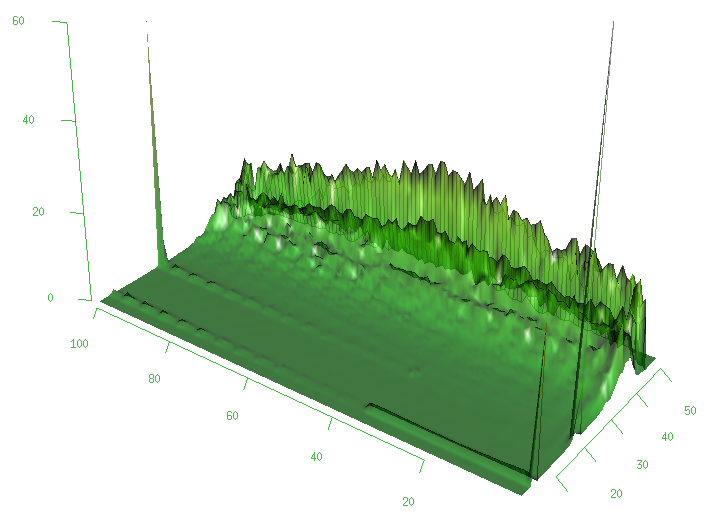
\includegraphics[width=9.5cm]{basequal_visible_cropped.png}
\end{center}
\caption{3-D Histogram of base qualities over read length for a sample BAM
  file. The x-axis (values range 1 to 100) shows the index of bases in the
  read, while the y-axis shows base quality. The z-axis is the scaled
  frequency. The plot was generated by converting the output of {\tt
    basequal\_stats.pig} using {\tt tools/basequal\_stats2matrix.pl} and then
  plotted using {\tt tools/plot\_basequal\_stats.R}.}
\label{fig:basequal3d}
\end{figure}

\subsubsection{Collecting per-base statistics of base qualities for reads}
Analogously to the previous example collecting statistics for the read bases, we can also collect
frequencies for base qualities conditioned on the position of the base inside
the reads. If these fall off too quickly for later positions, it may
indicate some quality issues with the run. The resulting script is actually
fairly similar to the previous one with the difference of not grouping
over the reference bases.
\begin{lstlisting}
run scripts/filter_defs.pig
A = load 'input.bam' using BamLoader('yes');
B = FILTER A BY not ReadUnmapped(flags) and not IsDuplicate(flags);
C = FOREACH B GENERATE ReadSplit(name,start,read,cigar,basequal,flags,mapqual,refindex,refname,attributes#'MD');
D = FOREACH C GENERATE FLATTEN($0);
base_stats_data = FOREACH D GENERATE basepos, basequal;
base_stats_grouped = GROUP base_stats_data BY (basepos, basequal);
base_stats_grouped_count = FOREACH base_stats_grouped GENERATE group.$0 as basepos, group.$1 AS basequal, COUNT($1) AS qcount;
base_stats_grouped = GROUP base_stats_grouped_count BY basepos;
base_stats = FOREACH base_stats_grouped {
        TMP1 = FOREACH base_stats_grouped_count GENERATE basequal, qcount;
        TMP2 = ORDER TMP1 BY basequal;
        GENERATE group, TMP2;
}
STORE base_stats into 'outputfile_basequalstats.txt';
\end{lstlisting}
Here is an example output (for a BAM file with 50 reads):
\begin{lstlisting}
0       {(37,10),(42,1),(51,20),(52,1),(59,1),(61,1),(62,1),(67,2),(68,2),(70,2),(71,4),(72,3),(73,1),(75,2)}
1       {(53,1),(56,1),(61,1),(63,1),(64,1),(65,2),(67,4),(68,3),(69,2),(70,7),(71,3),(72,3),(73,1),(74,4),(75,2),(76,5),(77,6),(78,2),(80,1)}
2       {(45,1),(46,1),(51,2),(57,1),(61,1),(65,2),(66,3),(67,2),(69,3),(71,4),(72,2),(73,6),(74,7),(75,1),(76,8),(77,2),(78,3),(80,1)}
3       {(58,1),(59,1),(60,1),(61,1),(62,1),(64,1),(65,2),(67,2),(68,1),(69,5),(70,1),(71,3),(72,7),(73,2),(74,4),(75,6),(76,2),(77,4),(78,3),(79,1),(81,1)}
4       {(55,1),(60,1),(61,1),(62,1),(64,1),(66,1),(67,3),(68,2),(69,1),(70,7),(71,2),(72,1),(73,4),(74,2),(75,2),(76,2),(77,2),(78,3),(79,7),(80,4),(81,2)}
5       {(51,1),(52,2),(54,1),(58,2),(62,2),(63,1),(66,3),(68,4),(70,1),(71,1),(72,2),(73,3),(74,1),(75,8),(76,1),(77,5),(78,1),(79,6),(80,3),(81,3)}
...
\end{lstlisting}
\begin{description}
	\item[Note] This example script is equivalent to executing from the command line
\begin{lstlisting}
$ seqpig -param inputfile=input.bam -param outputfile=outputfile_basequalstats.txt $SEQPIG_HOME/scripts/basequal_stats.pig
\end{lstlisting}
\end{description}

\subsubsection{Filtering reads by mappability threshold}
The script {\tt filter\_mappability.pig} filters reads in a given BAM file based on a given
mappability threshold. Both input BAM and mappability file need to reside inside HDFS.
\begin{lstlisting}
$ seqpig -param inputfile=/user/hadoop/input.bam -param outputfile=/user/hadoop/output.bam -param regionfile=/user/hadoop/mappability.100kbp.txt -param threshold=90 $SEQPIG_HOME/scripts/filter_mappability.pig
\end{lstlisting}
Note that since the script relies on distributing the BAM file header and the
mappability file via Hadoop's distributed cache, it is not possible to run it
with Pig in local mode.

\subsection{Processing Qseq and Fastq data}

SeqPig supports the import and export of non-aligned reads stored in
Qseq and Fastq data. Due to Pig's model that all records correspond to
tuples, which form bags, reads can be processed in very much the same
way independent of, for example, whether they are stored in Qseq or
Fastq. Also, since Fastq and Qseq files are header-less, there is no
pre-processing step required prior to loading the files, compared to
SAM/BAM import.

\subsubsection{Converting Qseq to Fastq and vice versa}

The following two lines simply convert an input Qseq file into Fastq format.
\begin{lstlisting}
reads = load 'input.qseq' using QseqLoader();
STORE reads INTO 'output.fastq' using FastqStorer(); 
\end{lstlisting}
The other direction works analogously.

The following examples are not specific to the type of input data
(Fastq, Qseq, BAM, $\ldots$). They roughly correspond to the ones
computed by the popular FastQC tool and can be all found in the {\tt
  fast\_fastqc.pig} script.

\subsubsection{Computing a read length distribution}
\label{sect:read_length_dist}

Once a read set is imported, it is fairly straightforward to compute
simple statistics, such as a histogram of the length of reads. Using
the {\tt LENGTH} string function, which is part of the PiggyBank (see
Section~\ref{sect:piggybank_note}), we can first compute the set of read
lengths, group them by their value and then compute the size of each
of the groups.

\begin{lstlisting}
DEFINE LENGTH org.apache.pig.piggybank.evaluation.string.LENGTH();
reads = load 'input.fq' using FastqLoader();
read_len = FOREACH reads GENERATE LENGTH(sequence);
read_len_counts = FOREACH (GROUP read_len BY $0) GENERATE group AS len, COUNT_STAR($1) as count;
\end{lstlisting}

\subsubsection{Computing a distribution of the average base quality of a read}

By using a SeqPig UDF to split reads into bases, one can compute this
statistic by relying on Pig's GROUP BY operator as follows.
%
\begin{lstlisting}
reads = load 'input.fq' using FastqLoader();
reads_by_bases = FOREACH reads GENERATE UnalignedReadSplit(sequence, quality);
read_q = FOREACH reads_by_bases GENERATE ROUND(AVG($0.basequal)) as read_qual;
read_q_counts = FOREACH (GROUP read_q BY read_qual) GENERATE group as avg_read_qual, COUNT_STAR($1) as count;
\end{lstlisting}

Alternatively, SeqPig also provides another UDF that has better performance
for larger read sets.
%
\begin{lstlisting}
reads = load 'input.fq' using FastqLoader();
read_seq_qual = FOREACH reads GENERATE quality;
avgbase_qual_counts = FOREACH (GROUP read_seq_qual ALL) GENERATE AvgBaseQualCounts($1.$0);
formatted_avgbase_qual_counts = FOREACH avgbase_qual_counts GENERATE
    FormatAvgBaseQualCounts($0);
\end{lstlisting}

\subsubsection{Distribution of GC content over the read set}

The following example shows how one can exploit Pig's GROUP and COUNT
operators to obtain statistics of the composition of read bases.

\begin{lstlisting}
reads = load 'input.fq' using FastqLoader();
reads_by_bases = FOREACH reads GENERATE UnalignedReadSplit(sequence, quality);
read_gc = FOREACH reads_by_bases {
  only_gc = FILTER $0 BY readbase == 'G' OR readbase == 'C';
  GENERATE COUNT(only_gc) as count;
}
read_gc_counts = FOREACH (GROUP read_gc BY count) GENERATE group as gc_count, COUNT_STAR($1) as count;
\end{lstlisting}

\subsubsection{Computing base statistics over the read set}

\label{sect:base_stats}

Similarly to GC content, one can rely on Pig operations to compute for
each read position the distribution of nucleotides and their base
qualities, as given by the aligner. However, in order to improve
performance for larger data sets, SeqPig also provides UDF's for this
purpose.

\begin{lstlisting}
reads = load 'input.fq' using FastqLoader();
read_seq_qual = FOREACH reads GENERATE sequence, quality;
base_qual_counts = FOREACH (GROUP read_seq_qual ALL) GENERATE BaseCounts($1.$0), BaseQualCounts($1.$1);
formatted_base_qual_counts = FOREACH base_qual_counts GENERATE FormatBaseCounts($0), FormatBaseQualCounts($1);
base_gc_counts = FOREACH base_qual_counts GENERATE FormatGCCounts($0);
\end{lstlisting}

\begin{description}
	\item[Note] All the statistics computed by the examples of Sections~\ref{sect:read_length_dist}--\ref{sect:base_stats} can be executed at once via
\begin{lstlisting}
$ seqpig -param inputpath=input.fq -param outputpath=fast-fastqc-output $SEQPIG_HOME/scripts/fast_fastqc.pig
\end{lstlisting}
\end{description}

\subsubsection{Clipping bases and base qualities}

\label{sect:read_clipping}

Assuming there were some problems in certain cycles of the sequencer,
it may be useful to clip bases from reads. This example removes the
last 3 bases and their qualities and stores the data under a new
filename. Note that here we rely on the {\tt SUBSTRING} and {\tt LENGTH}
string functions, which are part of the PiggyBank (see
Section~\ref{sect:piggybank_note}).

\begin{lstlisting}
DEFINE SUBSTRING org.apache.pig.piggybank.evaluation.string.SUBSTRING();
DEFINE LENGTH org.apache.pig.piggybank.evaluation.string.LENGTH();
reads = load 'input.qseq' using QseqLoader();
B = FOREACH A GENERATE instrument, run_number, flow_cell_id, lane, tile, xpos, ypos, read, qc_passed, control_number, index_sequence, SUBSTRING(sequence, 0, LENGTH(sequence) - 3) AS sequence, SUBSTRING(quality, 0, LENGTH(quality) - 3) AS quality;
store B into 'output.qseq' using QseqStorer();
\end{lstlisting}
\begin{description}
	\item[Note] This example script is equivalent to executing from the command line
\begin{lstlisting}
$ seqpig -param inputfile=input.qseq -param outputfile=output.qseq -param backclip=3 $SEQPIG_HOME/scripts/clip_reads.pig
\end{lstlisting}
\end{description}

\section{Performance tuning}

\subsection{Pig parameters}

Recent releases of Pig (such as 0.11.0) have a parameter that enables
aggregation of partial results on the mapper side, which greatly
improves performances of some of the UDF's described above. Further,
another option that is worth considering is to use so-called
\emph{schema tuples}. For more information see the Pig
documentation. The recommended setting is as follows:
\begin{itemize}
\item {\tt set pig.exec.mapPartAgg true;}
\item {\tt set pig.exec.mapPartAgg.minReduction 5;}
\item {\tt set pig.schematuple on;}
\end{itemize}

\subsection{Hadoop parameters}

Some scripts (such as {\tt pileup2.pig}) require an amount of memory that
depends on the choice of command line parameters. To tune the performance of
such operations on the Hadoop cluster,
consider the following Hadoop-specific parameters in {\tt mapred-site.xml}.
\begin{itemize}
\item {\tt mapred.tasktracker.map.tasks.maximum}: \\the maximum number simultaneous map tasks per worker node
\item {\tt mapred.tasktracker.reduce.tasks.maximum}:\\ the maximum number simultaneous reducer tasks per worker node
\item {\tt mapred.child.java.opts}:\\ Java options passed to child virtual
	machines at the worker nodes; for instanced, this may be used to configure
	the Java heap size to 1GB with {\tt -Xmx1000M}
\end{itemize}
Additionally, it is possible to pass command line parameters (such as mapper and reducer memory limits).
For instance, consider the Pig invocation (see {\tt tools/tun\_all\_pileup2.sh})
\begin{lstlisting}
${PIG_HOME}/bin/pig -Dpig.additional.jars=${SEQPIG_HOME}/lib/hadoop-bam-5.0.jar:${SEQPIG_HOME}/build/jar/SeqPig.jar:${SEQPIG_HOME}/lib/seal.jar:${SEQPIG_HOME}/lib/picard-1.76.jar:${SEQPIG_HOME}/lib/sam-1.76.jar -Dmapred.job.map.memory.mb=${MAP_MEMORY} -Dmapred.job.reduce.memory.mb=${REDUCE_MEMORY} -Dmapred.child.java.opts=-Xmx${CHILD_MEMORY}M -Dudf.import.list=fi.aalto.seqpig -param inputfile=$INPUTFILE -param outputfile=$OUTPUTFILE -param pparallel=${REDUCE_SLOTS} ${SEQPIG_HOME}/scripts/pileup2.pig
\end{lstlisting}
By setting appropriate values for {\tt MAP\_MEMORY, REDUCE\_MEMORY,
CHILD\_MEMORY} and for the number of available reduce slots {\tt REDUCE\_SLOTS}
one may be able to improve performance.

\subsection{Compression}

For optimal performance and space usage it may be advisable to enable the compression of
Hadoop map (and possibly reduce) output, as well as temporary data generated
by Pig. Compression with Pig can be enabled by setting properties such as
\begin{lstlisting}
  -Djava.library.path=/opt/hadoopgpl/native/Linux-amd64-64
  -Dpig.tmpfilecompression=true -Dpig.tmpfilecompression.codec=lzo
  -Dmapred.output.compress=true
  -Dmapred.output.compression.codec=org.apache.hadoop.io.compress.GzipCodec
\end{lstlisting}
on the Pig command line or the Hadoop configuration. Note that currently not all
Hadoop compression codecs are supported by Pig.  The details regarding which
compression codec to use depend are beyond the scope of this manual.


\end{document}
